\newpage
\section{State of the Implementation}

\subsection{Implementation Structure and Capabilities}

In order to demonstrate the capabilities of the OceanX system, we developed simulation software that modelled shipping operations both with and without our offshore smart ports and autonomous fleet. We ensured that system components were modelled in a realistic fashion by leveraging real world data, and considering a range of externalities. This allowed us to conduct an accurate quantitative evaluation of the advantages of our model compared to the freight shipping industry as it exists today.

Our solution architecture is composed of three logically distinct tiers: back-end, front-end, and data. The back-end, a Java web application server, contains all business logic related to the simulation and is responsible for correctly and accurately modelling the movement of ships and their interactions with ports. In order to ensure that the simulation is ecologically valid, it uses shipping lane data from a custom dataset hosted on the Mapbox web service. Using this data, the back-end software is able to create a graph whose edges represent the paths that ships are able to take. Information relating to the simulation, such as the location of containers and the velocities of ships, is then served via websockets to the React/Deck.gl front-end for rendering. Our front-end system then uses this information to appropriately display the positions and statuses of all ships and ports in the system.

The simulation itself is executed on a `tick-by-tick’ basis, where a tick can be described as the software’s atomic time unit. Each entity in the system is assigned one of several possible agent types, which determines how the agent behaves and moves. Our possible agent types include autonomous ships, freight ships, coastal ports, and offshore ports. On each tick of the system, every agent is provided the ‘world’ as it appeared in the previous tick. From this, agents are expected to determine an appropriate action. This decentralised control system models collaborative autonomy. It provides more redundancy and resiliency than would be possible with a single monolithic controller, where a single point of failure could disrupt the entire system. The speed of the simulation is controlled by a speed scaling factor that can be set by the user. This factor is used to modify the speed of operations such as ship movement or cargo loading or unloading. 

Figure \ref{fig:class_diagram} shows a class diagram detailing all classes used by the backend. Several key classes from the system that provide fundamental functionality in regard to the simulation are briefly outlined below. 

\begin{description}
	\item[JSONable] An interface that requires the implementation of the \texttt{toJSON} method. Used to serialise the world and its constituent agents for transfer to the front-end Javascript.
	\item[Agent] Provides the abstract method \lstinline{tick} that all agents within the system are required to implement in order to define their behaviour. Each agent possesses an ID, an agent type and a set of coordinates defining its location. Every agent implements \lstinline{JSONable}.
	\item[Simulation] Ticks the world and all agents that it contains in time with the number of ticks per second specified. Responsible for sending the state of the world to the front-end.
\end{description}

\newpage
\begin{figure}[h!]
	\centering
	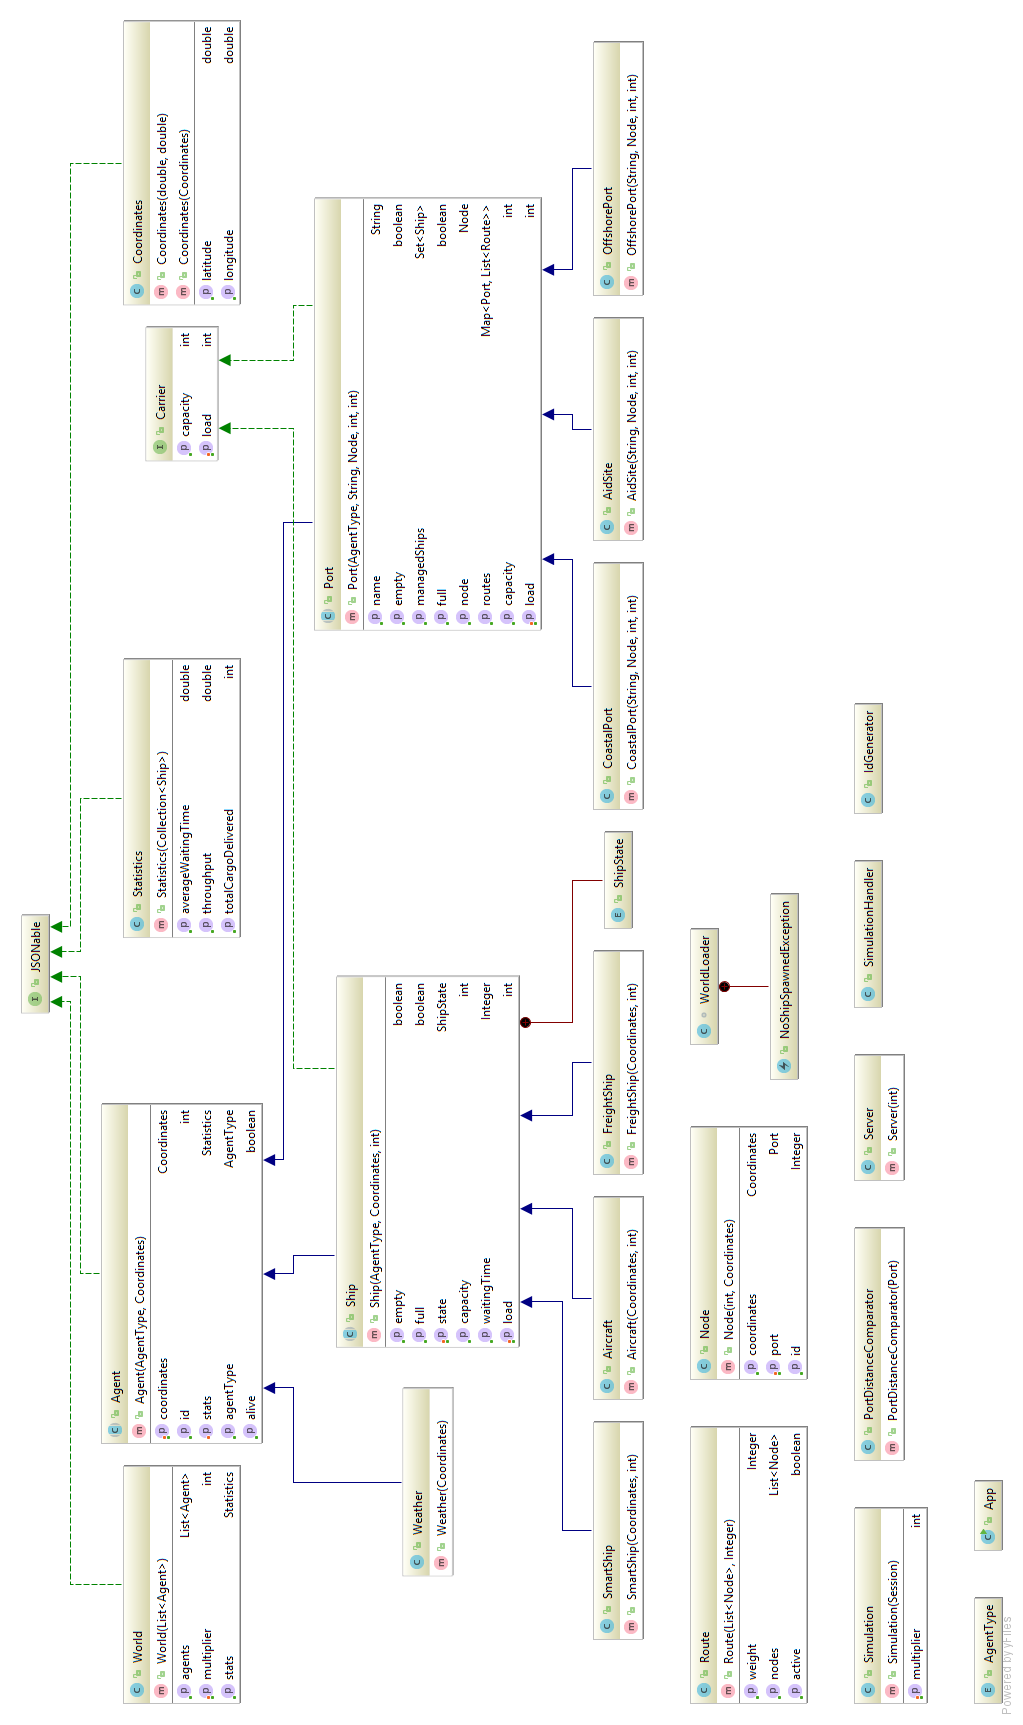
\includegraphics[height=0.93\textheight]{images/class_diagram}
	\caption{Class diagram detailing all classes used by the backend.}
	\label{fig:class_diagram}
\end{figure}



\newpage
In order to make sure our model was accurate, we had to implement many of the processes that ships would have to follow in a real-world system. For example, we included a mechanism by which ports could request collection of cargo from nearby idle ships. This collaborative process is essential in ensuring that containers are able to flow efficiently through the system. For this purpose, we developed a heuristic algorithm capable of establishing the most suitable ship for collecting cargo awaiting transport. Specifically, idle ships servicing the port at which this cargo is based are required to submit a `bid’ detailing their suitability to collect the cargo. Each bid is a trade-off between the capacity of the ship and the number of containers that require collection. A ship that could collect all cargo but has a large amount of empty space is penalised, with the system instead favouring ships that can be utilized more efficiently. If all nearby ships are occupied, the port will instead request idle ships from other ports that are connected to it by shipping routes. Allowing each ship to create its own bid allows for a much more flexible system than one controlled centrally, which fundamentally increases the reliability of the overall system.

Our simulation engine allowed us to compare the OceanX system with traditional shipping operations. In order to achieve this, we built a separate shipping lane dataset that did not contain the offshore ports, again fetched from the Mapbox web service by the Java back-end. We developed and integrated a comprehensive statistics suite, which collects and displays information pertaining to the performance of both the OceanX and legacy systems. It is based on these statistics that we reached informed conclusions as to the benefits our system can attain. The statistics we collected include:

\begin{itemize}[noitemsep]
	\item the total number of containers moved;
	\item the throughput, or number of containers moved per time tick;
	\item the average waiting time at ports.
\end{itemize}

\subsection{Future Work}

By designing, implementing, and evaluating these control mechanisms now, we have reduced the future work required to develop the system to an initially deployable state. We have ensured that the low-level detail and functionality of the system is sound, and we have verified that it improves on the existing shipping industry methodology through quantitative testing.

We would need to invest a significant amount of time, effort and capital to develop both the hardware and software required to develop the system into an initially deployable state. Firstly, we would need to design and construct the autonomous shuttle ships, including the communication and navigation software that enables ship-to-ship and ship-to-port communication. Using this software, we could design mechanisms for collision and danger avoidance systems. Software for the control of the cargo collection and storage systems is fundamental to the automatic functionality of the offshore ports, but we do not currently consider this as part of the simulation. This software would determine how containers are automatically unloaded, stored, and routed to their onward destination when they are ready to leave the port.

Further to this, we need to develop software to control the docking procedure for shuttle ships with coastal and offshore ports. This software would take advantage of the communication capabilities of the ship to interface with these ports, allowing the efficient transfer of cargo. Finally, we must consider procedures for the handling of shuttle ship breakdowns, failure, or power loss. This functionality would mitigate the risk of losing hardware by ensuring that these ships are recoverable and serviceable following unforeseen hardware or software failure.
